\section*{Question 6}
In this question we will redo the portfolio analysis of the previous question, but this time we will use the historical average to predict the future returns and use two different methods to estimate the variance. The first method is calculating the sample variance over the past 60 months ($RW$) and the second method is the $GARCH(1,1)$ model ($GARCH$)over the expanding window from the beginning of the sample to the current month. 

     We used the same method as in question 4 to calculate the optimal weights of the portfolios. The results are shown in the following figures. 
     Our calculation for the utility gain shows that the utility gain of the $GARCH$ model is $0.0029$ and the $RW$ model is $0.006$ with respect to the historical average. 
     We can see that the $GARCH$ model has a better performance than the $RW$ model but due to the higher volatility of the $GARCH$ portfolio the utility gain is lower than the $RW$ model.




    \begin{figure}[htbp!]
        \centering
        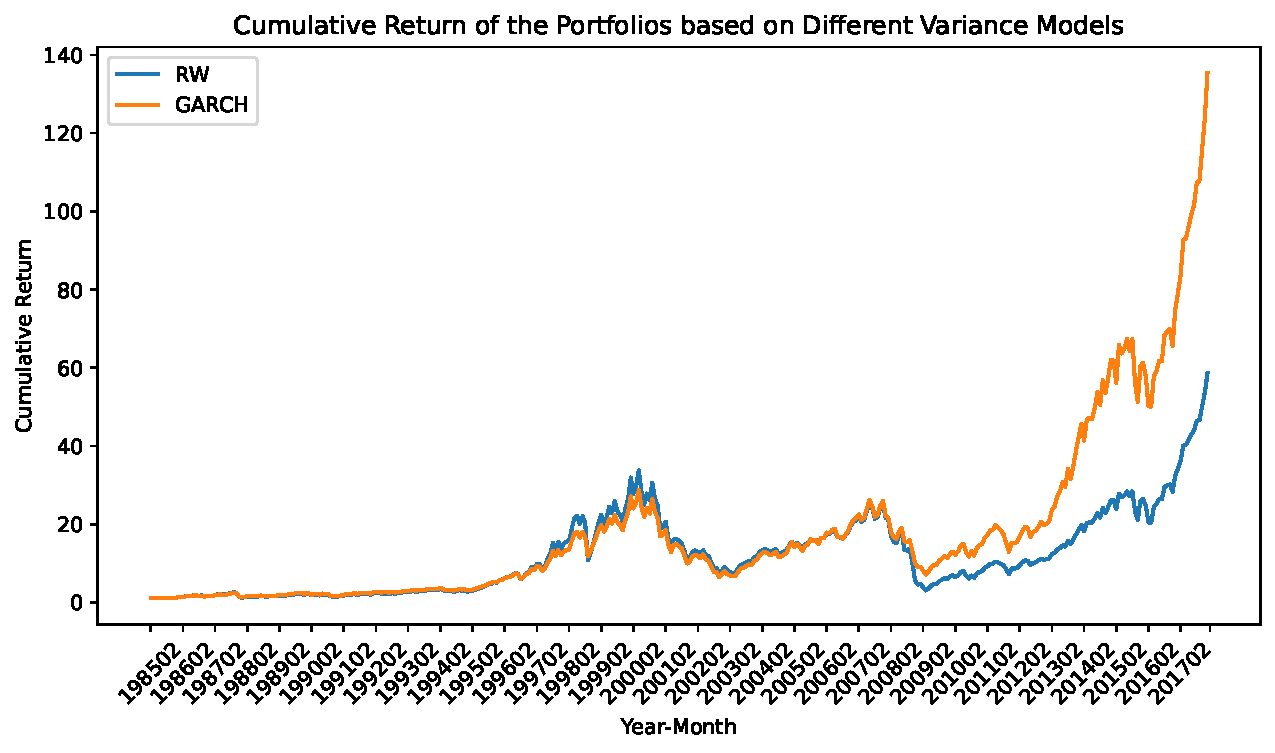
\includegraphics[width=0.75\textwidth]{Out/Ex6_C.pdf}
        \caption{Optimal weights of the portfolios}
    \end{figure}
    

    \begin{figure}[htbp!]
        \centering
        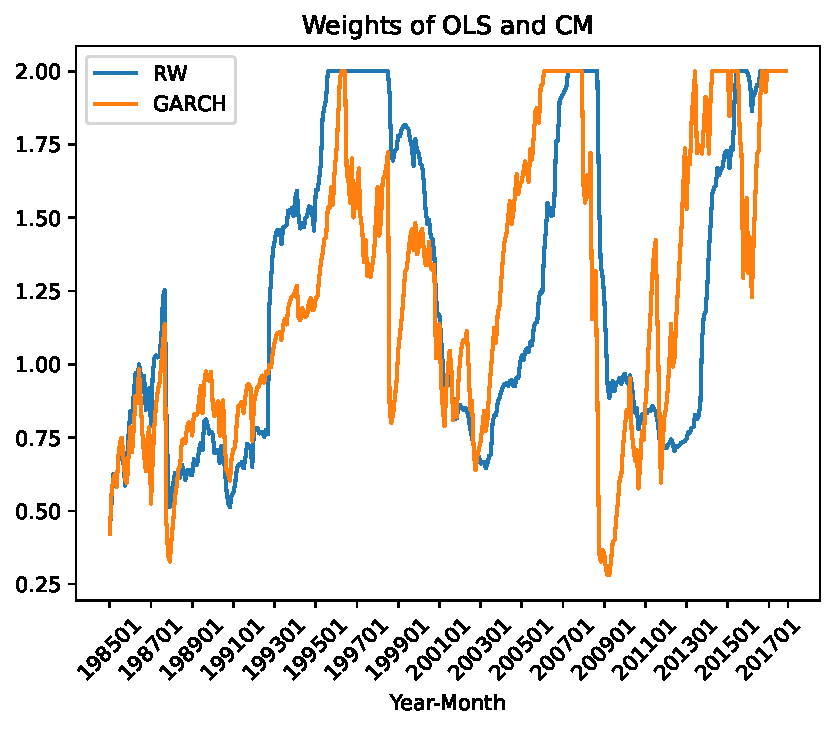
\includegraphics[width=0.65\textwidth]{Out/Ex6_D.pdf}
        \caption{Optimal weights of the portfolios}
    \end{figure}

